%% 
%% Copyright 2019 Elsevier Ltd
%% 
%%
%%%%%%%%%%%%%%%%%%%%%%%%%%%% ! ! ! SUBMISSION CHECKLIST ! ! ! %%%%%%%%%%%%%%%%%%%%%%%%%%%%
%%
%% Please confirm that your submission follows all the requirements of the guidelines, including the submission checklist:
%% _ Code availability section 
%% _ Highlights
%% _ Authorship statement
%% _ Cover letter
%% _ The manuscript must be single column and double spaced
%% _ Reference must be in the author-date format
%%
%% *All the masnucripts in disagreement with the guidelines will be desk-rejected without editorial check.
%%
%% --------------------------------------
%%
%% This file is part of the 'CAS Bundle'.
%%  
%% It may be distributed under the conditions of the LaTeX Project Public
%% License, either version 1.2 of this license or (at your option) any
%% later version.  The latest version of this license is in 
%%    http://www.latex-project.org/lppl.txt 
%% and version 1.2 or later is part of all distributions of LaTeX
%% version 1999/12/01 or later.
%%   
%% The list of all files belonging to the 'CAS Bundle' is
%% given in the file `manifest.txt'.
%% 
%% Template article for cas-dc documentclass for  
%% double column output.
 
%\documentclass[a4paper,fleqn,longmktitle]{cas-dc}
\documentclass[a4paper,fleqn]{cas-sc}

\usepackage[authoryear]{natbib}
\usepackage{graphicx} 
\usepackage{float}
\usepackage{algorithm}  
\usepackage{algpseudocode}
\usepackage{color}
\usepackage{setspace}
\usepackage[nomarkers,figuresonly]{endfloat}


\newcommand{\colorComments}{black} 
 
%%%Author definitions
\def\tsc#1{\csdef{#1}{\textsc{\lowercase{#1}}\xspace}}
\tsc{WGM}
\tsc{QE}
\tsc{EP}
\tsc{PMS}
\tsc{BEC}
\tsc{DE}
%%%

\usepackage{lineno}
\linenumbers 

\begin{document}
\let\WriteBookmarks\relax
\def\floatpagepagefraction{1}
\def\textpagefraction{.001}
\shorttitle{Short title}
\shortauthors{short author name}

\title [mode = title]{Manuscript title - \LaTeX  template for Computers \& Geosciences  }


\author[1]{Author 1}[type=editor,
                        auid=000,bioid=1,orcid=0000-0000-0000-0000]
\credit{ Author 1 contribution  }

\author[2]{Author 2} 
\credit{Author 2 contribution }

\author[3]{Author 3}
\credit{Author 3 contribution}

%\cormark[2]
%\fnmark[1,3]

\address[1]{Author 1 affiliation}
\address[2]{Author 2 affiliation}
\address[3]{Author 3 affiliation} 

\begin{abstract}
Abstract text here, abstract text here,  abstract text here,  abstract text here,  abstract text here,  abstract text here,  abstract text here,  abstract text here,  abstract text here,  abstract text here,  abstract text here,  abstract text here,  abstract text here,  abstract text here,  abstract text here,  abstract text here,  abstract text here,  abstract text here,  abstract text here,  
\end{abstract}
 
\begin{coverletter}

Dear Editors,
\newline
 
please find the enclosed manuscript entitled as "..." which we are submitting for exclusive consideration for publication as an article in Computers \& Geosciences. We confirm that our submission follows all the pre-review requirements including all the item of the submission checklist.  
\newline
 
The manuscript presents a new algorithm for ..... 
\newline

We provide the source codes in a public repository that can be found in the section "Code availability".
\newline

Thank you for your consideration of our work. 
\newline

Sincerely,
\newline

Authors names

Author 1 e-mail
\newline

\textbf{Delete before submission:}

Please confirm that your submission follows all the requirements of the guidelines, including the submission checklist:

- Code availability section 

- Highlights

- Authorship statement

- Cover letter

- The manuscript must be single column and double spaced

- Reference must be in the author-date format

*All the masnucripts in disagreement with the guidelines will be desk-rejected without editorial check.



\end{coverletter}

 
\begin{highlights}
\item Highlight 1
\item Highlight 2
\item Highlight 3
\item Highlight 4
\item Highlight 5
\end{highlights}

\begin{keywords}
Keyword 1 \sep Keyword 2 \sep Keyword 3 \sep Keyword 4
\end{keywords}

\maketitle 

\doublespacing

\textbf{Code availability section}

Name of the code/library

Contact: e-mail and phone number

Hardware requirements: ...

Program language: ...
 
Software required: ...

Program size: ...

The source codes are available for downloading at the link:
https://github.com/ . . . . 

\section{Introduction}
\label{intro}



Example of citation:

\cite{DEFIGUEIREDO2021, Tran1994, JaimeGmezHernndez1990,pardo2003connec3d, hansen2018multiple, CAGEO_2019_mingliang, CAGEO_2004_GSTAT_Slanguage}

Example of citation with parentheses: 

\citep{DEFIGUEIREDO2021, Tran1994, JaimeGmezHernndez1990,pardo2003connec3d, hansen2018multiple, CAGEO_2019_mingliang, CAGEO_2004_GSTAT_Slanguage}

\section{Methodology}

Example of equations:
\begin{equation}
\label{eqn:cumulative_definition}
    P( z_{j}^l |z_{1}^l,...,z_{j-1}^l) = \int_{-\infty}^{z_{j}^l} p(z_j|z_{1}^l,...,z_{j-1}^l) dz_j = u.
\end{equation}


\subsection{Subsection}

\begin{equation} 
\label{eqn:sampling_from_inverse_cumulative_2}
    z_j(x_i) = P^{-1}( \Phi( g_j(x_i) )|z_1(x_i),...,z_{j-1}(x_i))
\end{equation}

\section{Algorithm and implementation}

Example of algorithm:
\begin{algorithm}
  \caption{DMS for generating $n$ spatially correlated variables with dimension ($m\times1$) from a generic (non-parametric) joint distribution }
  
  \begin{algorithmic}
  \label{alg:integrado}
  \State \textbf{Input 1} Non-parametric distribution given by a ($k \times n$)-matrix $\boldsymbol{o}$ with $k$ observations of $n$ variables;
  \State \textbf{Input 2} Theoretical correlation function $\boldsymbol{\lambda}$ for the $n$ variables to be simulated;
  \newline
  
 %\Statex \textit{1.}  $\boldsymbol{O} = $KDE$(\boldsymbol{O})$; 
 %\Comment{\textit{Optional: Expand observed data using KDE if necessary}}
 
 \Statex \textit{1.} $\boldsymbol{g}$ = FFTMAA($\lambda$); \Comment{\textit{Generate a $(m\times n)$-matrix with $n$ Gaussian realizations with $m$ components by FFTMA}}
  \Statex \textit{2.} $\boldsymbol{u} = \overline{\Phi}(\boldsymbol{g})$;
 \Comment{\textit{Compute a $(m\times n)$-matrix with $n$ uniformly distributed simulations with $m$ components}}
 \State \textit{3.}  $P_1$ = $\overline{P}(z_{1})$ from observed data $\boldsymbol{o}$;
 \Comment{\textit{Compute the cumulative distribution of the first variable}}
  \newline
   \For{ i = 1,..., m}
   \State \textit{4.} $\boldsymbol{z}_{1}^l(x_i)$ = \textit{interpolate}($P_1$, $\Omega_1$, $\boldsymbol{u}_{1}(x_i)$);
   \Comment{\textit{Apply the inverse of $P_1$ to $\boldsymbol{u}_{1}(x_i)$} in the discretized domain $\Omega_1$}
   \For{ j = 2,..., n} 
   \State \textit{5.}  $P_j$ = $\overline{P}$($z_j$|$\boldsymbol{z}_{1}^{l}(x_i),...,\boldsymbol{z}_{j-1}^{l}(x_i)$ ) from observed data $\boldsymbol{O}$; \Comment{{Compute the cumulative distribution of the variable $z_j$ conditioned to the drawn values $\boldsymbol{z}_{1}^{l}(x_i),...,\boldsymbol{z}_{j-1}^{l}(x_i)$}}
   \State \textit{6.} $\boldsymbol{z}_{j}^{l}(x_i)$ = \textit{interpolate}($P_j$, $\Omega_j$, $\boldsymbol{u}_{j}^l(x_i)$); 
   \Comment{\textit{Apply the inverse of $P_j$ to $\boldsymbol{u}_{j}(x_i)$} in the discretized domain $\Omega_j$}
  \EndFor
  \EndFor 
  \newline
\State  \textbf{Output:} ($m \times n$)-matrix $\boldsymbol{z}$ with $n$ spatially correlated realizations with $m$ components following the joint distribution of the observed data $\boldsymbol{o}$;
  \end{algorithmic} 
\end{algorithm} 


\section{Results}


Example of figure

\begin{figure}
\centering
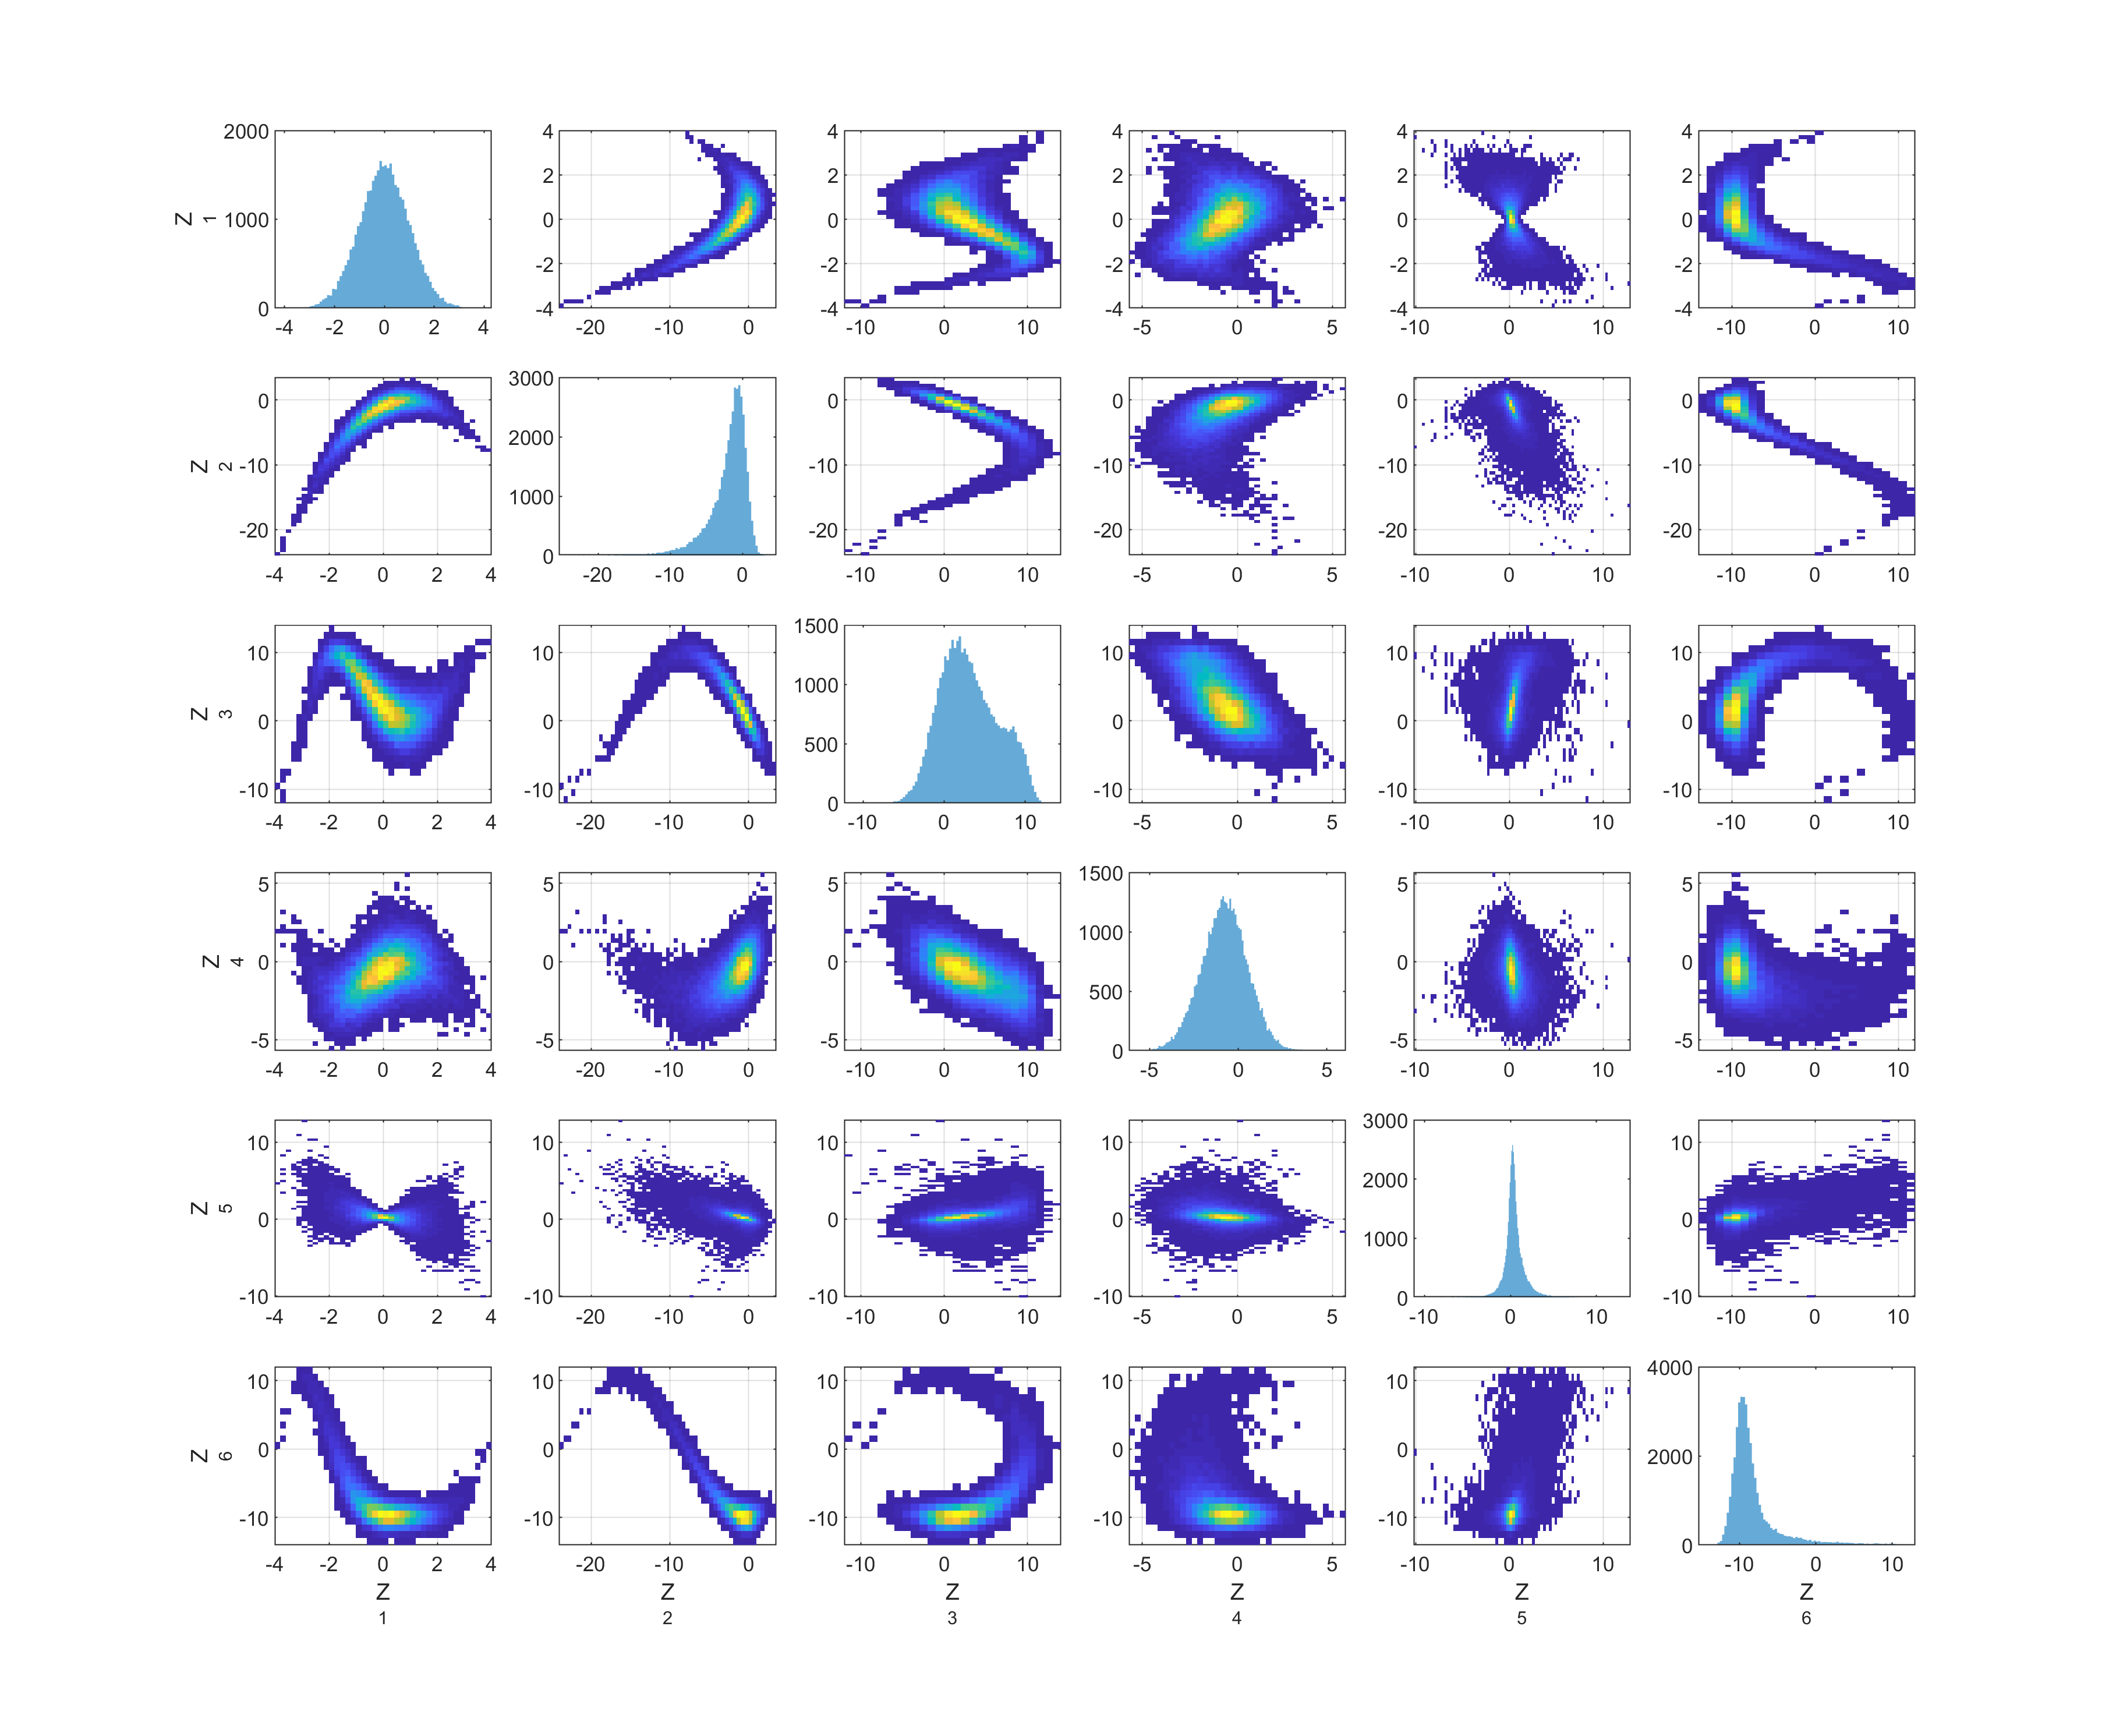
\includegraphics[width=0.75\textwidth]{figs_rev1/uncond_distribution_reference.png}
\caption{ Reference 6-variate non-parametric PDF. The histograms along the diagonal represent the marginal distributions of the variables in the sequential order $z_1,...,z_6$, and the bivariate histograms represent the bivariate marginal distributions of the variables. }
\label{fig:uncond_distribution_reference}
\end{figure}

Example of table:

\begin{table}
\centering
\caption{Mean squared errors of the experimental histograms and bi-variate distributions of the unconditional simulation obtained by DMS and the reference distribution.}
\label{tab:dms}
\begin{tabular}{ |c||c|c|c|c|c|c| } 
 \hline
     & $z_1$  &  $z_2$  &  $z_3$  &  $z_4$  &  $z_5$  &   $z_6$\\ 
 \hline 
 \hline
$z_1$ & 0.000014 &  0.20    &   0.13   &  0.075  &  0.25    &	0.1 \\
\hline
$z_2$ & 0.20    &   0.17    &   2.46   &   0.12  &  0.9	    &   0.27 \\
\hline
$z_3$ & 0.13    &   2.5     &   0.31   &  0.09   &	0.23    &   0.18\\
\hline 
$z_4$ & 0.075   &	0.12    &  0.089   &  0.21   &   0.13   &   0.13\\
\hline
$z_5$ & 0.25    &   0.88    &   0.26   &  0.13   &   0.18   &   0.22\\
\hline
$z_6$ & 0.10    &   0.27    &   0.18   &  0.13   &   0.22   &   0.38\\
\hline
\end{tabular} 
\end{table}


\subsection{Subsection}


\section{Conclusion}

Conclusion here...

\section{Acknowledgments}

The authors would like to acknowledge ...

\printcredits

\bibliographystyle{cas-model2-names}
\bibliography{bibliography} 

\end{document}

